\documentclass[10pt,letterpaper]{article}
\usepackage[spanish,es-tabla,es-nodecimaldot]{babel}
\usepackage[utf8]{inputenc}
\usepackage[T1]{fontenc}
\usepackage{lmodern}
\usepackage{amsmath,amssymb,amsfonts}
\usepackage{graphicx}
\usepackage{textcomp}
\usepackage{xcolor}
\usepackage{booktabs}
\usepackage{float}
\usepackage{placeins}
\usepackage{rotating}
\usepackage{array}
\usepackage{siunitx}
\sisetup{output-decimal-marker={.},group-separator={\,},group-minimum-digits=4,detect-all}
\usepackage{url}
\usepackage{xurl}
\usepackage{etoolbox}
\usepackage{caption}
\captionsetup{font=small,labelfont=bf}
\AtBeginEnvironment{thebibliography}{\raggedright}
\usepackage{geometry}
\geometry{letterpaper,left=25mm,right=25mm,top=30mm,bottom=25mm}
\usepackage{fancyhdr}
\pagestyle{fancy}
\fancyhf{}
\rhead{EL-5854 Sistemas Fotovoltaicos}
\lhead{ITCR $\vert$ Escuela de Ingeniería Electrónica}
\rfoot{Pág.\ \thepage}
\lfoot{II Semestre 2026}
\setlength{\headheight}{14pt}
\graphicspath{{figuras/}}
\newlength{\anchofig}\setlength{\anchofig}{0.72\textwidth}
\newcommand{\kwhmd}{kWh/(m\textsuperscript{2}$\cdot$día)}
\newenvironment{IEEEkeywords}{\par\smallskip\noindent\textbf{Palabras clave:} }{\par}
\renewcommand{\thetable}{\arabic{table}}

\renewcommand{\topfraction}{0.9}
\renewcommand{\bottomfraction}{0.8}
\renewcommand{\textfraction}{0.07}
\renewcommand{\floatpagefraction}{0.75}
\setcounter{topnumber}{3}
\setcounter{bottomnumber}{2}
\setcounter{totalnumber}{4}
\let\figorig\figure \let\endfigorig\endfigure
\renewenvironment{figure}[1][]{\figorig[!htbp]}{\endfigorig}
\let\taborig\table \let\endtaborig\endtable
\renewenvironment{table}[1][]{\taborig[!htbp]}{\endtaborig}
\renewenvironment{figure*}[1][]{\begin{figure}}{\end{figure}}
\renewenvironment{table*}[1][]{\begin{table}}{\end{table}}

\begin{document}

\title{Diseño de un sistema fotovoltaico aislado de respaldo para las cargas críticas de una vivienda en Santa Rosa de Oreamuno}
\author{A. López, S. Rojas, J. Segura\\[2pt]
\small Escuela de Ingeniería Electrónica, Instituto Tecnológico de Costa Rica}
\date{II Semestre 2026}
\thispagestyle{fancy}
\maketitle
\thispagestyle{fancy}

\begin{abstract}
En este proyecto se diseñó un sistema fotovoltaico aislado que respalda las cargas críticas de una vivienda en Santa Rosa de Oreamuno, Cartago, servida por JASEC. Las cargas críticas son el refrigerador, el congelador, la iluminación, los cargadores de celular y de laptop y el módem, que consumen \SI{4.33}{kWh} por día. Con el procedimiento del curso, dos días de autonomía, un banco de \SI{24}{V} y una profundidad de descarga de 70\,\%, se requieren \SI{758}{Ah}, que se cubren con cuatro baterías LiFePO\textsubscript{4} Power Queen de \SI{24}{V} y \SI{200}{Ah} en paralelo. El generador tiene cuatro módulos AIKO de \SI{450}{W} (\SI{1.8}{kWp}) en dos cadenas de dos, sobre la cara este del techo, inclinada \SI{12}{\degree}, con un regulador MPPT Victron SmartSolar 150/85 y un inversor-cargador Victron MultiPlus-II de \SI{3000}{VA} con transferencia automática. Incluso en noviembre, el mes de menor radiación, la energía disponible cubre el 116\,\% de la demanda. El diseño incluye la estructura, el cableado, las protecciones y el diagrama unifilar. El precio estimado es de ¢7.10 millones; el sistema reduce la factura anual en ¢128\,165 (54\,\%), pero con los reemplazos de equipos y baterías la inversión no se recupera en 25 años, por lo que su justificación es la continuidad del servicio y no el ahorro.
\end{abstract}

\begin{IEEEkeywords}
sistema fotovoltaico aislado, respaldo, baterías LiFePO\textsubscript{4}, regulador MPPT, inversor-cargador
\end{IEEEkeywords}

\section{Introducción}

El objetivo de este proyecto es diseñar un sistema fotovoltaico aislado que mantenga en funcionamiento las cargas críticas de la vivienda de Abner López, en Santa Rosa de Oreamuno, cuando falla el servicio eléctrico. La vivienda tiene servicio de JASEC, por lo que el sistema se planteó como respaldo: las cargas críticas se alimentan desde un subtablero propio, normalmente con energía solar y el banco de baterías, y la red queda como apoyo. El banco se dimensionó para dos días de autonomía.

El diseño sigue el procedimiento de sistemas aislados del curso: caracterización del consumo, recurso solar, balance de energía, banco de baterías, generador fotovoltaico, regulador de carga e inversor. Parte de los datos de placa de los equipos de la casa, de la factura de JASEC, de la base de datos PVGIS y de las fichas técnicas de los equipos seleccionados.

\section{Descripción del lugar de estudio}\label{sec:lugar}

\subsection{Ubicación y características de la zona}

La vivienda está en Santa Rosa, distrito del cantón de Oreamuno, en la provincia de Cartago. La Tabla~\ref{tab:sitio} resume la información general del sitio y la Fig.~\ref{fig:satelital} muestra su ubicación.

\begin{table}[!htb]
\caption{Información general del sitio}
\label{tab:sitio}
\centering
\footnotesize
\setlength{\tabcolsep}{3pt}
\begin{tabular}{l l}
\toprule
Parámetro & Valor \\
\midrule
Ubicación & Santa Rosa, Oreamuno, Cartago \\
Coordenadas & \ang{9;56;9.04}\,N, \ang{83;49;38.23}\,O \\
Elevación & \SI{2317}{m} s.\,n.\,m. \\
Distribuidora y tarifa & JASEC, residencial (T-RE) \\
Techo & Lámina de zinc ondulada, a dos aguas \\
Inclinación y orientación & \SI{12}{\degree} hacia el este y \SI{12}{\degree} hacia el oeste \\
Área del techo en planta & \SI{85}{m^2} (perímetro de \SI{36.8}{m}) \\
Temperatura ambiente, últimos 12 meses & mínima \SI{7}{\celsius}, máxima \SI{29.5}{\celsius} (abril de 2026) \\
\bottomrule
\end{tabular}
\\[2pt]
{\footnotesize Elevación según PVGIS \cite{pvgis}, que coincide con la de Google Earth sobre el techo (\num{2313} a \SI{2315}{m}); coordenadas y área medidas en Google Earth. Techo y temperaturas: datos de los propietarios de la vivienda.}
\end{table}

\begin{figure}[!htb]
\centering
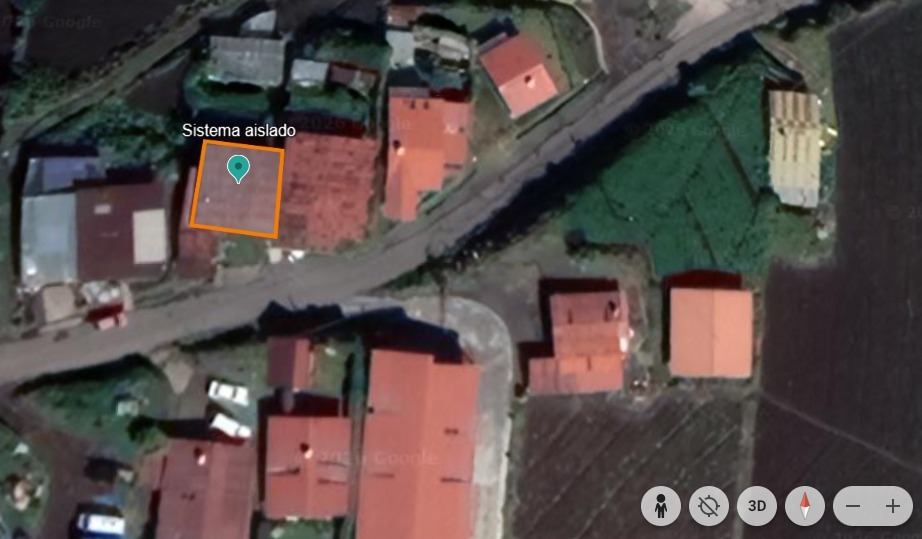
\includegraphics[width=\anchofig]{ubicacion_satelital.jpg}
\caption{Ubicación de la vivienda en Santa Rosa de Oreamuno (imagen de Google Earth). El recuadro marca el techo.}
\label{fig:satelital}
\end{figure}

El sitio está en las faldas del volcán Irazú, a \SI{2317}{m} de altura, en una zona de viviendas rodeada de terrenos de cultivo, como se observa en la Fig.~\ref{fig:satelital}. Por la altura, el clima es frío: en los últimos doce meses la temperatura varió entre 7 y \SI{29.5}{\celsius}. La temperatura media mensual de PVGIS está entre 16.3 y \SI{18.6}{\celsius} (Sección~\ref{sec:recurso}). En la imagen satelital no se identifican edificaciones ni árboles más altos junto a la cara este del techo; la ausencia de sombras debe confirmarse en el sitio.

El techo es de lámina de zinc ondulada, a dos aguas, con la cumbrera en dirección norte--sur, de modo que una cara mira al este y la otra al oeste, ambas con \SI{12}{\degree} de inclinación. En planta mide unos \SI{85}{m^2}, aproximadamente \SI{9.2}{m} por lado, de modo que cada cara tiene unos \SI{4.6}{m} de ancho horizontal (\SI{4.7}{m} sobre la pendiente) y \SI{9.2}{m} de largo.

\subsection{Caracterización del consumo}

\subsubsection{Cargas críticas}

Se levantó la lista de los equipos de la casa con sus horas de uso y se tomaron los datos de placa de los principales. Con el dueño se definieron como cargas críticas las que deben seguir funcionando si falla el servicio: la refrigeración de alimentos, la iluminación y las comunicaciones. Quedaron fuera la ducha eléctrica, la cocina, el microondas, la lavadora y la cámara de refrigeración. La Tabla~\ref{tab:cargas} presenta las cargas críticas y la Fig.~\ref{fig:consumo_equipos}, su energía diaria.

\begin{table*}[!htb]
\caption{Cargas críticas de la vivienda}
\label{tab:cargas}
\centering
\footnotesize
\setlength{\tabcolsep}{3pt}
\begin{tabular}{l c c c c c c c r}
\toprule
Equipo & Cant. & $V$ [V] & $P_{\mathrm{nom}}$ [W] & $P_{\mathrm{pico}}$ [W] & $I_{\mathrm{nom}}$ [A] & $I_{\max}$ [A] & Horas/día & Energía [Wh/día] \\
\midrule
Refrigerador Atlas AC12SSAAWA & 1 & 115 & 196.7 & 786.8\textsuperscript{a} & 1.71 & 6.84\textsuperscript{a} & 9 & 1770.3 \\
Congelador Daytron MCHF90 & 1 & 115 & 130.0 & 520.0\textsuperscript{a} & 1.20 & 4.80\textsuperscript{a} & 10 & 1300.0 \\
Cargadores de celular (5)\textsuperscript{b} & 1 & 120 & 35.0 & 175.0 & 0.29 & 1.46 & 12 & 420.0 \\
Cargadores de laptop (3)\textsuperscript{c} & 1 & 120 & 51.7 & 155.1 & 0.43 & 1.29 & 6 & 310.2 \\
Bombillos LED Sylvania A60 & 3 & 120 & 15.0 & 15.0 & 0.13 & 0.13 & 5 & 225.0 \\
Bombillos LED Sylvania A60 & 4 & 120 & 15.0 & 15.0 & 0.13 & 0.13 & 2 & 120.0 \\
Bombillo LED Sylvania A60 & 1 & 120 & 15.0 & 15.0 & 0.13 & 0.13 & 3 & 45.0 \\
Módem Nexxt Nebula N300 & 1 & 120 & 6.0 & 6.0 & 0.05 & 0.05 & 24 & 144.0 \\
\midrule
\multicolumn{8}{l}{Total (todas las cargas en CA, 120 V)} & 4334.5 \\
\bottomrule
\end{tabular}
\\[2pt]
{\footnotesize Datos de placa y de la lista de equipos (noviembre de 2026). Donde la placa no da la tensión se usa \SI{120}{V}, y la corriente se calcula como $P/V$.
\textsuperscript{a}Supuesto: arranque del compresor de 4 veces la potencia nominal, el valor alto del intervalo típico de 3 a 4 veces.
\textsuperscript{b}Cargadores de 40, 35, 35, 45 y \SI{20}{W}; se usa la potencia media de \SI{35}{W} con 12 horas de carga en total, y como pico los cinco a la vez (\SI{175}{W}).
\textsuperscript{c}Delta de \SI{45.1}{W}, Lenovo de \SI{65.0}{W} y HP de \SI{45.0}{W}; potencia media de \SI{51.7}{W} con 6 horas en total, y como pico los tres a la vez.}
\end{table*}

\begin{figure}[!htb]
\centering
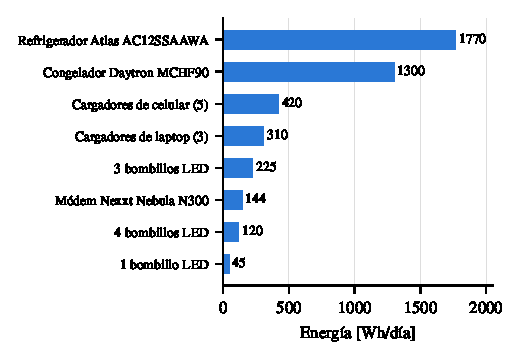
\includegraphics[width=\anchofig]{consumo_equipos.pdf}
\caption{Energía diaria de las cargas críticas.}
\label{fig:consumo_equipos}
\end{figure}

Las cargas críticas consumen \SI{4334.5}{Wh} por día, todas en corriente alterna a \SI{120}{V}. El refrigerador y el congelador suman \SI{3070}{Wh}, el 71\,\% del total. Si todas las cargas se encienden a la vez, incluidos los cinco cargadores de celular y los tres de laptop, la potencia es de \SI{783}{W}; si además arrancan los dos compresores, el pico llega a \SI{1763}{W}. Estos dos valores se usan para seleccionar el inversor.

\subsubsection{Consumo de la vivienda}

Se cuenta con la factura de JASEC de octubre de 2026, por ¢19\,175, y se sabe que las facturas han estado entre ¢16\,000 y ¢22\,000. Con la tarifa residencial de JASEC para 2026 \cite{aresep_tre}, el alumbrado público \cite{aresep_ap}, el tributo de bomberos (1.75\,\% del cargo de energía cuando se superan \SI{100}{kWh}) \cite{ley8992} y el IVA (13\,\% del cargo de energía cuando se superan \SI{280}{kWh}) \cite{ley9635}, la factura de octubre corresponde a \SI{275}{kWh}. La Tabla~\ref{tab:tarifa} resume la tarifa.

\begin{table}[!htb]
\caption{Tarifa residencial de JASEC (T-RE) para 2026}
\label{tab:tarifa}
\centering
\footnotesize
\begin{tabular}{l r}
\toprule
Cargo & Valor \\
\midrule
Energía, primeros \SI{30}{kWh} (cargo fijo) & ¢1863.30 \\
Energía, de 31 a \SI{200}{kWh} & ¢62.11/kWh \\
Energía, más de \SI{200}{kWh} & ¢76.02/kWh \\
Alumbrado público, primeros \SI{30}{kWh} & ¢80.10 \\
Alumbrado público, más de \SI{30}{kWh} & ¢2.67/kWh \\
Bomberos (más de \SI{100}{kWh}) & 1.75\,\% del cargo de energía \\
IVA (más de \SI{280}{kWh}) & 13\,\% del cargo de energía \\
\bottomrule
\end{tabular}
\\[2pt]
{\footnotesize Las facturas se redondean al múltiplo de ¢5 más cercano.}
\end{table}

Como solo se tiene una factura, los demás meses se estimaron con la variación mensual de un ejemplo de facturación de una vivienda servida por JASEC: los meses que en el ejemplo superan a octubre conservan la misma proporción, y en los que quedan por debajo la diferencia con octubre se redujo para que el mes más bajo diera unos ¢16\,100. Diciembre, que es el mes de mayor consumo de la casa, se igualó al mes más alto del resto del año. El resultado está en la Tabla~\ref{tab:facturas} y en la Fig.~\ref{fig:facturas}: \SI{3230}{kWh} y ¢236\,730 al año, con facturas de ¢16\,135 a ¢22\,495. Las cargas críticas representan el 49\,\% del consumo anual de la casa.

\begin{table}[!htb]
\caption{Consumo y factura mensual estimados para 2026}
\label{tab:facturas}
\centering
\footnotesize
\setlength{\tabcolsep}{4pt}
\begin{tabular}{l r r r r}
\toprule
Mes & Casa [kWh] & Cargas críticas [kWh] & Factura actual [¢] & Factura con el sistema [¢] \\
\midrule
Ene & 237.0 & 134.4 & 16\,135 & 6\,760 \\
Feb & 256.1 & 121.4 & 17\,665 & 8\,875 \\
Mar & 281.0 & 134.4 & 22\,070 & 9\,660 \\
Abr & 257.8 & 130.0 & 17\,800 & 8\,415 \\
May & 276.3 & 134.4 & 19\,280 & 9\,350 \\
Jun & 283.7 & 130.0 & 22\,315 & 10\,120 \\
Jul & 241.4 & 134.4 & 16\,485 & 7\,050 \\
Ago & 285.7 & 134.4 & 22\,495 & 9\,970 \\
Set & 281.9 & 130.0 & 22\,150 & 10\,005 \\
Oct\textsuperscript{a} & 275.0 & 134.4 & 19\,175 & 9\,265 \\
Nov & 268.6 & 130.0 & 18\,665 & 9\,125 \\
Dic & 285.7 & 134.4 & 22\,495 & 9\,970 \\
\midrule
Total & 3230.2 & 1582.1 & 236\,730 & 108\,565 \\
\bottomrule
\end{tabular}
\\[2pt]
{\footnotesize \textsuperscript{a}Factura real. Los demás meses son estimados. La factura con el sistema se explica en la Sección~\ref{sec:economia}.}
\end{table}

\begin{figure}[!htb]
\centering
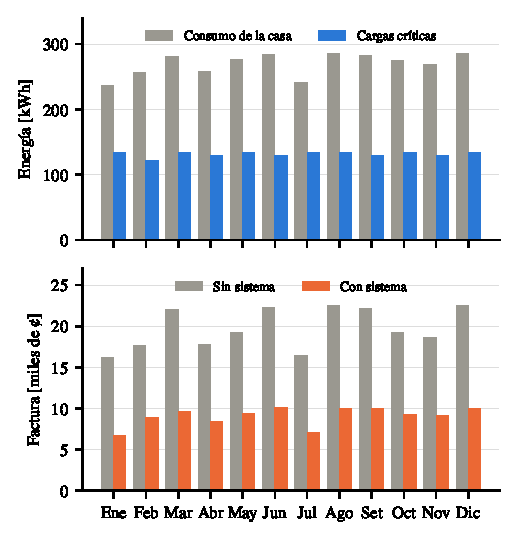
\includegraphics[width=\anchofig]{consumo_facturas.pdf}
\caption{Consumo mensual de la casa y de las cargas críticas (arriba) y factura sin y con el sistema (abajo).}
\label{fig:facturas}
\end{figure}

\section{Recurso solar}\label{sec:recurso}

\subsection{Diagrama cilíndrico}

La posición del Sol se calculó con la declinación $\delta$, el ángulo horario $\omega=15^\circ(t_s-12)$, donde $t_s$ es el tiempo solar, y la latitud $\phi=\SI{9.936}{\degree}$:
\begin{equation}
\sin h = \sin\phi\,\sin\delta + \cos\phi\,\cos\delta\,\cos\omega,
\end{equation}
\begin{equation}
\sin\alpha = \frac{\cos\delta\,\sin\omega}{\cos h},
\end{equation}
donde $h$ es la altura solar y $\alpha$ el acimut medido desde el sur (en la figura se expresa desde el norte, en sentido horario). La Fig.~\ref{fig:cilindrico} presenta el diagrama cilíndrico del sitio para el día 21 de cada mes.

\begin{figure*}[!t]
\centering
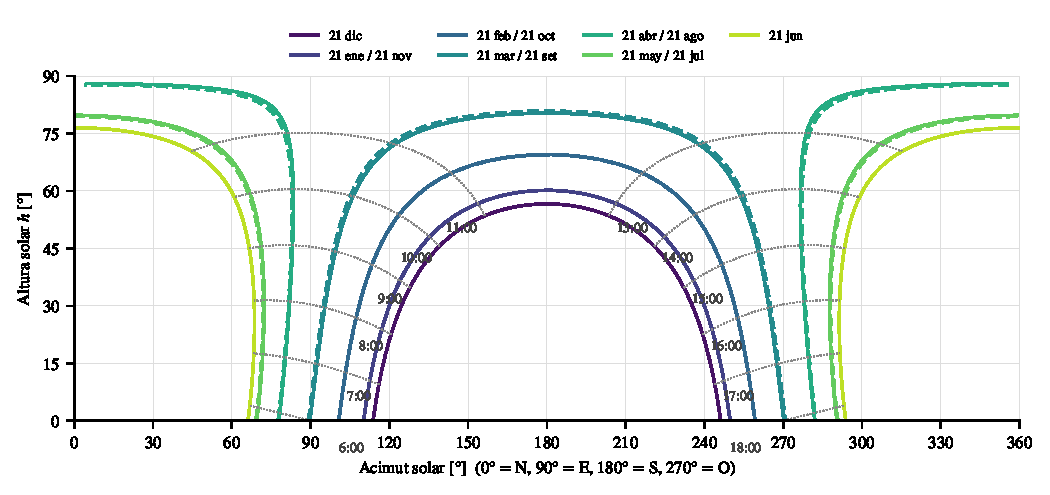
\includegraphics[width=0.95\textwidth]{diagrama_cilindrico.pdf}
\caption{Diagrama cilíndrico del recorrido solar en Santa Rosa de Oreamuno (\SI{9.936}{\degree}\,N), día 21 de cada mes, en tiempo solar. Las líneas punteadas unen puntos de la misma hora.}
\label{fig:cilindrico}
\end{figure*}

Por la cercanía al ecuador, el Sol pasa alto todo el año: al mediodía solar la altura es de \SI{56.6}{\degree} el 21 de diciembre, la menor del año, y de \SI{80.3}{\degree} el 21 de marzo. Entre abril y agosto el Sol pasa al norte del cenit y en el resto del año, al sur. El día dura entre \SI{11.4}{h} y \SI{12.6}{h}. Como el Sol sale por el este todo el año, la cara este del techo recibe sol directo desde el amanecer, y la cara oeste desde el mediodía.

\subsection{Radiación solar}

La radiación se obtuvo de PVGIS 5.3, con la base PVGIS-ERA5 de 2005 a 2023 y el horizonte calculado con el modelo de elevación del terreno \cite{pvgis}. Se consultó la irradiación sobre el plano horizontal, sobre las dos caras del techo (\SI{12}{\degree} al este y \SI{12}{\degree} al oeste), sobre un plano de \SI{12}{\degree} al sur y sobre el plano óptimo que calcula PVGIS. La Tabla~\ref{tab:radiacion} presenta los promedios diarios de cada mes, expresados en horas solares pico (HSP), y la Fig.~\ref{fig:radiacion} los grafica.

\begin{table}[!htb]
\caption{Irradiación diaria media por mes [HSP = kWh/(m$^2\cdot$día)] y temperatura media}
\label{tab:radiacion}
\centering
\footnotesize
\setlength{\tabcolsep}{3.5pt}
\begin{tabular}{l c c c c c c}
\toprule
Mes & Horizontal & \SI{12}{\degree} este & \SI{12}{\degree} oeste & \SI{12}{\degree} sur & Óptimo & $T_{\mathrm{media}}$ [\si{\celsius}] \\
\midrule
Ene & 5.02 & 5.03 & 4.88 & 5.59 & 5.56 & 16.3 \\
Feb & 5.69 & 5.73 & 5.50 & 6.11 & 6.12 & 16.5 \\
Mar & 5.88 & 5.94 & 5.65 & 6.01 & 6.07 & 17.1 \\
Abr & 5.47 & 5.54 & 5.23 & 5.34 & 5.43 & 18.1 \\
May & 4.44 & 4.55 & 4.22 & 4.22 & 4.35 & 18.6 \\
Jun & 4.24 & 4.36 & 4.02 & 3.99 & 4.11 & 18.6 \\
Jul & 4.28 & 4.35 & 4.08 & 4.05 & 4.15 & 18.2 \\
Ago & 4.41 & 4.51 & 4.18 & 4.26 & 4.37 & 18.3 \\
Set & 4.38 & 4.49 & 4.14 & 4.38 & 4.48 & 18.4 \\
Oct & 3.85 & 3.94 & 3.66 & 4.00 & 4.06 & 18.2 \\
Nov & 3.68 & \textbf{3.73} & 3.54 & 3.97 & 3.98 & 17.5 \\
Dic & 4.45 & 4.46 & 4.33 & 5.00 & 4.95 & 16.8 \\
\midrule
Año [kWh/m$^2$] & 1695 & 1721 & 1623 & 1728 & 1750 & \\
\bottomrule
\end{tabular}
\\[2pt]
{\footnotesize Fuente: PVGIS 5.3, PVGIS-ERA5 2005--2023 \cite{pvgis}. Óptimo: \SI{14}{\degree} de inclinación y acimut de \SI{-40}{\degree} (hacia el sureste).}
\end{table}

\begin{figure}[!htb]
\centering
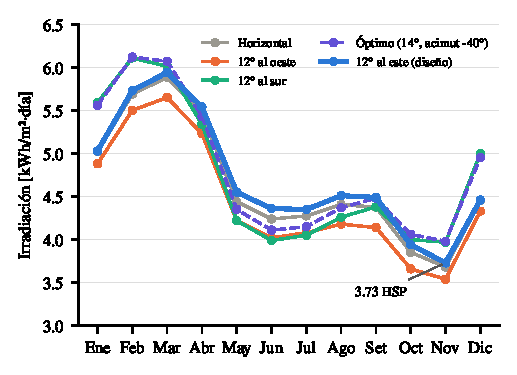
\includegraphics[width=\anchofig]{radiacion_mensual.pdf}
\caption{Irradiación diaria media por mes en distintos planos (PVGIS).}
\label{fig:radiacion}
\end{figure}

Se distinguen dos épocas: sobre la cara este, de diciembre a abril la irradiación diaria está entre 4.46 y \SI{5.94}{HSP}, y de mayo a noviembre baja a valores de 3.73 a \SI{4.55}{HSP}, con el mínimo en noviembre. En ese periodo la fracción difusa media de PVGIS sube de 0.26--0.34 a 0.43--0.49, lo que corresponde a la época lluviosa \cite{pvgis}.

\subsection{Ángulo óptimo y plano de diseño}

PVGIS calcula como óptimo un plano de \SI{14}{\degree} de inclinación con acimut de \SI{-40}{\degree}, que recibe \SI{1750}{kWh/m^2} al año \cite{pvgis}. La cara este del techo, con \SI{12}{\degree}, recibe \SI{1721}{kWh/m^2}, solo 1.7\,\% menos, y la cara oeste \SI{1623}{kWh/m^2}, 5.6\,\% menos que la cara este. Por eso los módulos se colocan en la cara este, paralelos al techo: una estructura que los orientara al óptimo ganaría 1.7\,\% de energía a cambio de más material y más carga de viento sobre la lámina.

En un sistema aislado el dimensionamiento se hace con el mes de menor radiación, porque el banco debe recargarse también en ese mes. Sobre la cara este ese mes es noviembre, con \SI{3.73}{HSP}. En noviembre el plano óptimo recibiría \SI{3.98}{HSP}, 6.7\,\% más, pero la diferencia no cambia la cantidad de módulos (Sección~\ref{sec:aislado}).

\section{Módulo fotovoltaico}\label{sec:modulo}

\subsection{Descripción del módulo}

Se seleccionó el módulo AIKO Neostar 2S AIKO-A450-MAH54Mb, de \SI{450}{W}, por su eficiencia de 22.6\,\%, su bajo coeficiente de temperatura de potencia (\SI{-0.26}{\%/\celsius}) y su baja degradación garantizada, de 1\,\% el primer año y 0.35\,\% por año después \cite{aiko_ds}. Es de silicio monocristalino tipo n con celdas ABC (\emph{all back contact}), con los dos contactos en la cara posterior, de modo que la cara frontal no tiene rejilla metálica que haga sombra sobre la celda. Tiene 108 medias celdas, vidrio templado de \SI{3.2}{mm}, marco de aluminio y tres diodos de paso \cite{aiko_ds}.

\subsection{Características eléctricas}

La Tabla~\ref{tab:modulo} reúne los datos de la ficha técnica en condiciones estándar de prueba (STC) y NOCT.

\begin{table}[!htb]
\caption{Características del módulo AIKO-A450-MAH54Mb \cite{aiko_ds}}
\label{tab:modulo}
\centering
\footnotesize
\setlength{\tabcolsep}{3pt}
\begin{tabular}{l c c}
\toprule
Parámetro & STC & NOCT \\
\midrule
Potencia máxima, $P_{\max}$ & \SI{450}{W} & \SI{339}{W} \\
Tensión de máx. potencia, $V_{mp}$ & \SI{33.70}{V} & \SI{31.83}{V} \\
Corriente de máx. potencia, $I_{mp}$ & \SI{13.36}{A} & \SI{10.66}{A} \\
Tensión de circuito abierto, $V_{oc}$ & \SI{40.69}{V} & \SI{38.43}{V} \\
Corriente de cortocircuito, $I_{sc}$ & \SI{14.12}{A} & \SI{11.42}{A} \\
\midrule
Eficiencia del módulo & \multicolumn{2}{c}{22.6\,\%} \\
Coef. de temperatura de $P_{\max}$ & \multicolumn{2}{c}{\SI{-0.26}{\%/\celsius}} \\
Coef. de temperatura de $V_{oc}$ & \multicolumn{2}{c}{\SI{-0.22}{\%/\celsius}} \\
Coef. de temperatura de $I_{sc}$ & \multicolumn{2}{c}{\SI[retain-explicit-plus]{+0.05}{\%/\celsius}} \\
Tensión máxima del sistema & \multicolumn{2}{c}{\SI{1500}{V} CC} \\
Fusible máximo en serie & \multicolumn{2}{c}{\SI{25}{A}} \\
Dimensiones & \multicolumn{2}{c}{\SI{1757}{} $\times$ \SI{1134}{} $\times$ \SI{30}{mm}} \\
Masa & \multicolumn{2}{c}{\SI{21.5}{kg}} \\
Cable de salida & \multicolumn{2}{c}{\SI{4}{mm^2} (12 AWG), conector MC4} \\
\bottomrule
\end{tabular}
\\[2pt]
{\footnotesize STC: \SI{1000}{W/m^2}, \SI{25}{\celsius} en la celda, AM 1.5. NOCT: \SI{800}{W/m^2}, \SI{20}{\celsius} ambiente, viento de \SI{1}{m/s}.}
\end{table}

\subsection{Variación de los parámetros con la temperatura}

La temperatura de la celda se estimó con
\begin{equation}
T_{\mathrm{celda}} = T_{\mathrm{amb}} + \frac{\mathrm{NOCT}-20}{800}\,G,
\label{eq:tcelda}
\end{equation}
donde $G$ es la irradiancia en \si{W/m^2}. La ficha no da la temperatura NOCT de la celda, por lo que se estimó con los valores NOCT de la Tabla~\ref{tab:modulo}: con \SI{800}{W/m^2} y la celda a \SI{25}{\celsius} el módulo daría \SI{360}{W}, y para que la potencia baje a \SI{339}{W} la celda debe estar a \SI{47.4}{\celsius}; con la corriente se obtiene \SI{47.0}{\celsius}. Se usó un NOCT de \SI{47}{\celsius}.

La temperatura mínima de la celda se tomó igual a la mínima ambiente, \SI{7}{\celsius}, porque al amanecer, con poca irradiancia, la celda está a la temperatura del aire. Para la máxima se usó la ambiente máxima de \SI{29.5}{\celsius} con $G=\SI{1000}{W/m^2}$, lo que según \eqref{eq:tcelda} da \SI{63.2}{\celsius}. Cada parámetro se corrigió con
\begin{equation}
X(T) = X_{\mathrm{STC}}\left[1 + \frac{\gamma_X}{100}\,(T_{\mathrm{celda}} - 25)\right],
\label{eq:correccion}
\end{equation}
donde $\gamma_X$ es el coeficiente de temperatura del parámetro. La ficha no da coeficientes para $V_{mp}$ e $I_{mp}$: para $I_{mp}$ se usó el de $I_{sc}$, y para $V_{mp}$ se estimó $\gamma_{V_{mp}}\approx\gamma_{P}-\gamma_{I_{sc}}=\SI{-0.31}{\%/\celsius}$, de modo que el producto $V_{mp}\cdot I_{mp}$ concuerde con la potencia corregida. Este coeficiente es una aproximación y no un dato del fabricante. Los resultados están en la Tabla~\ref{tab:temperatura}.

\begin{table}[!htb]
\caption{Parámetros del módulo corregidos por temperatura (\SI{1000}{W/m^2})}
\label{tab:temperatura}
\centering
\small
\setlength{\tabcolsep}{4.5pt}
\begin{tabular}{l S[table-format=2.2] S[table-format=2.2] S[table-format=2.2] S[table-format=2.2] S[table-format=3.1]}
\toprule
{$T_{\mathrm{celda}}$} & {$V_{oc}$ [V]} & {$V_{mp}$ [V]} & {$I_{sc}$ [A]} & {$I_{mp}$ [A]} & {$P$ [W]} \\
\midrule
\SI{7}{\celsius} (mín.) & 42.30 & 35.58 & 13.99 & 13.24 & 471.1 \\
\SI{25}{\celsius} (STC) & 40.69 & 33.70 & 14.12 & 13.36 & 450.0 \\
\SI{63.2}{\celsius} (máx.) & 37.27 & 29.70 & 14.39 & 13.62 & 405.2 \\
\bottomrule
\end{tabular}
\end{table}

Entre los dos extremos, $V_{oc}$ varía en un 12.4\,\% de su valor en STC y $V_{mp}$ en un 17.4\,\%, mientras que la corriente cambia un 2.8\,\%. La potencia baja a \SI{405}{W} con la celda a \SI{63.2}{\celsius} y sube a \SI{471}{W} a \SI{7}{\celsius}. La tensión a \SI{7}{\celsius} limita la cantidad máxima de módulos en serie, la de \SI{63.2}{\celsius} la mínima, y la corriente a \SI{63.2}{\celsius} se usa para revisar el regulador y dimensionar los conductores.

\section{Banco de baterías}\label{sec:baterias}

Para seleccionar las baterías se compararon cinco modelos de ciclo profundo de dos tecnologías, plomo-ácido (inundada, AGM y gel) y LiFePO\textsubscript{4}, con un banco de \SI{24}{V} y una profundidad de descarga (DOD) de diseño de 70\,\%. Las Tablas~\ref{tab:opciones} y~\ref{tab:matriz} resumen las opciones y la matriz comparativa, con los datos de los fabricantes \cite{trojan_t105, trojan_sig, trojan_saes, ultracell, pq, victron_ds} y precios minoristas de Estados Unidos y Europa de noviembre de 2026. El costo por kWh útil se calculó como el precio entre la energía nominal multiplicada por la DOD, y el costo durante la vida útil como el costo por kWh útil entre los ciclos declarados.

\begin{table}[!htb]
\caption{Especificaciones de las opciones comerciales}
\label{tab:opciones}
\centering
\footnotesize
\setlength{\tabcolsep}{2.2pt}
\begin{tabular}{l l c c c c c}
\toprule
Ref. & Tecnología & $V$ [V] & $C$ [Ah] & Unid. 24\,V & Ciclos (DOD) & Masa [kg] \\
\midrule
B1 & Inundada & 6 & 225 & 4 & 1200 (50\,\%)\textsuperscript{a} & 28 \\
B2 & AGM & 12 & 179 & 2 & 1200 (100\,\%) & 57 \\
B3 & Gel\textsuperscript{b} & 12 & 206 & 2 & 1200 (50\,\%)\textsuperscript{a} & 62.2 \\
B4 & LiFePO\textsubscript{4} & 25.6 & 200 & 1 & 6000 (80\,\%) & 37.5 \\
B5 & LiFePO\textsubscript{4} & 25.6 & 200 & 1 & 2500 (80\,\%) & 39 \\
\bottomrule
\end{tabular}
\\[2pt]
{\footnotesize Capacidad a $C_{20}$ para B1 a B3. \textsuperscript{a}Dato de un documento del fabricante alojado por un distribuidor. \textsuperscript{b}Híbrida AGM y gel.}
\end{table}

\begin{table*}[!th]
\caption{Matriz comparativa de las baterías (módulo de \SI{24}{V})}
\label{tab:matriz}
\centering
\footnotesize
\setlength{\tabcolsep}{4pt}
\resizebox{\textwidth}{!}{%
\begin{tabular}{l r c c r r c r c >{\raggedright\arraybackslash}p{0.17\textwidth} r c}
\toprule
Ref. & Precio & $E_{\text{nom}}$ & DOD & \multicolumn{2}{c}{Costo por kWh útil [USD]} & Ciclos & $c_{\text{vida}}$ & Eficiencia & Mantenimiento & Masa & Garantía \\
\cmidrule(lr){5-6}
 & [USD] & [kWh] & tecnol. & DOD tecnol. & DOD 70\,\% & & [USD/kWh] & [\%] & & [kg] & [años] \\
\midrule
B1 & 900.00 & 5.40 & 50\,\% & 333 & 238 & 1200 & 0.28 & n.d. & Agua, ecualización, ventilación & 112 & 1\textsuperscript{a} \\
B2 & 1278.40 & 4.30 & 100\,\% & 298 & 425 & 1200 & 0.25 & n.d. & Ninguno; tensiones de carga AGM & 114 & 3\textsuperscript{b} \\
B3 & 807.25 & 4.94 & 50\,\% & 327 & 233 & 1200 & 0.27 & n.d. & Ninguno; tensiones de carga gel & 124 & n.d. \\
B4 & 809.99 & 5.12 & 80\,\% & 198 & 226 & 6000 & 0.03 & n.d. & Ninguno; BMS integrado & 38 & 5 \\
B5 & 2983.50 & 5.12 & 80\,\% & 728 & 832 & 2500 & 0.29 & 92 & Ninguno; requiere BMS externo de Victron & 39 & 3 \\
\bottomrule
\end{tabular}}
\\[2pt]
{\footnotesize Precio y masa del conjunto de unidades que forma \SI{24}{V}. n.d.: no declarado por el fabricante. El precio de B2 es el de oferta (\$639.20 por unidad) y no incluye flete.
\textsuperscript{a}Garantía de Trojan para América Latina, válida solo con DOD de hasta 50\,\%. \textsuperscript{b}Garantía de la línea AES; en Costa Rica debe confirmarse con el distribuidor.}
\end{table*}

Se seleccionó la batería B4, Power Queen LiFePO\textsubscript{4} de \SI{25.6}{V} y \SI{200}{Ah}. Tiene el menor costo por kWh útil del conjunto, \SI{198}{USD/kWh}, frente a 298, 327 y \SI{333}{USD/kWh} de las opciones de plomo-ácido (B2, B3 y B1) y \SI{728}{USD/kWh} de B5. También es la más barata con la DOD de 70\,\%: \SI{226}{USD/kWh} frente a 233 de B3, 238 de B1, 425 de B2 y 832 de B5. Declara 6000 ciclos al 80\,\% de DOD, frente a 1200 del plomo-ácido, por lo que su costo durante la vida útil es de \SI{0.03}{USD/kWh} con el precio de Estados Unidos y de \SI{0.08}{USD/kWh} con el de Costa Rica, frente a 0.25 a \SI{0.29}{USD/kWh} de las demás. Esta cifra la declara solo el fabricante, y B5 declara 2500 ciclos a la misma DOD. Aun con 2500 ciclos, B4 costaría \SI{0.08}{USD/kWh} con el precio de Estados Unidos y \SI{0.19}{USD/kWh} con el de Costa Rica, menos que las demás. La DOD de diseño, 70\,\%, queda dentro del 80\,\% al que se declaran sus ciclos.

Pesa \SI{7.3}{kg/kWh} nominal, frente a 21 a \SI{27}{kg/kWh} del plomo-ácido. Un banco de cuatro B4 pesa \SI{150}{kg}, frente a \SI{498}{kg} de ocho B3 y \SI{570}{kg} de diez B2. B5 es comparable, con \SI{7.6}{kg/kWh}. B4 no requiere mantenimiento, trae el BMS integrado y tiene cinco años de garantía del fabricante, que debe confirmarse con el distribuidor local.

El modelo se vende en Costa Rica en 850\,000 colones \cite{kuat}, precio que se usa en el presupuesto (Sección~\ref{sec:economia}). Hay dos condiciones que tomar en cuenta. La primera es que el banco usa las cuatro unidades en paralelo que admite el fabricante \cite{pq_manual}, de modo que no admite ampliaciones. La segunda es la temperatura: B4 se carga entre 0 y \SI{50}{\celsius} y no tiene protección de carga a baja temperatura \cite{pq}. En el sitio la temperatura mínima del último año fue de \SI{7}{\celsius} y la máxima de \SI{29.5}{\celsius}, dentro del intervalo de carga, y el banco se ubicará en un cuarto techado y ventilado junto al tablero principal, sin sol directo. El dimensionamiento del banco se presenta en la Sección~\ref{sec:balance}.

La batería seleccionada es de fosfato de hierro y litio (LiFePO\textsubscript{4}). Cada celda tiene \SI{3.2}{V} nominales, de modo que ocho celdas en serie forman la batería de \SI{25.6}{V}, que es la versión comercial de \SI{24}{V}; por eso el banco se dimensiona como de \SI{24}{V} \cite{linden}. Frente al plomo-ácido, admite descargas profundas con muchos más ciclos y no requiere mantenimiento, y su química es más estable térmicamente que la de otras baterías de ion-litio, con menor riesgo de incendio \cite{zubi2018}. Necesita un sistema de gestión (BMS) que equilibre las celdas y desconecte la batería por sobretensión, subtensión, sobrecorriente o temperatura fuera de rango, y no se debe cargar por debajo de \SI{0}{\celsius} \cite{linden}. La Tabla~\ref{tab:bateria} resume las características de la batería seleccionada.

\begin{table}[!htb]
\caption{Características de la batería Power Queen \SI{24}{V} \SI{200}{Ah} \cite{pq}}
\label{tab:bateria}
\centering
\footnotesize
\begin{tabular}{l l}
\toprule
Parámetro & Valor \\
\midrule
Química & LiFePO\textsubscript{4}, BMS de \SI{200}{A} integrado \\
Tensión nominal & \SI{25.6}{V} (8 celdas de \SI{3.2}{V}) \\
Capacidad y energía nominales & \SI{200}{Ah}, \SI{5120}{Wh} \\
Carga & CC/CV, \SI{28.8 \pm 0.4}{V} \\
Corriente de carga recomendada & \SI{40}{A} (0.2C) \\
Corriente continua máxima de carga y descarga & \SI{200}{A} \\
Potencia continua máxima & \SI{5120}{W} \\
Ciclos & 4000 (100\,\%), 6000 (80\,\%), 15\,000 (60\,\% de DOD) \\
Temperatura de carga & 0 a \SI{50}{\celsius} \\
Temperatura de descarga & $-20$ a \SI{60}{\celsius} \\
Conexión máxima & 4 en paralelo, 2 en serie \\
Resistencia interna & $\leq\SI{40}{m\ohm}$ \\
Protección & IP65 \\
Masa y dimensiones & \SI{37.5}{kg}, $520\times268\times\SI{220}{mm}$ \\
Garantía & 5 años \\
\bottomrule
\end{tabular}
\end{table}

\section{Diseño del sistema aislado}\label{sec:aislado}

\subsection{Configuración del sistema}

El sistema es de respaldo: las cargas críticas se trasladan a un subtablero que se alimenta desde la salida del inversor-cargador. El generador fotovoltaico carga el banco de baterías por medio de un regulador MPPT, y el inversor-cargador convierte la energía del banco a \SI{120}{V} de corriente alterna. La red de JASEC llega a la entrada de corriente alterna del inversor-cargador; si el banco llega a su descarga máxima, la red alimenta las cargas y puede recargar el banco, y si la red falla, el equipo pasa las cargas al inversor. El sistema no entrega energía a la red.

\subsection{Balance de energía y capacidad del banco}\label{sec:balance}

La energía que debe entregar el generador se calculó con el método de balance de energía para sistemas aislados:
\begin{equation}
E_T = \frac{E_{CC}}{K_{TCC}} + \frac{E_{CA}}{K_{TCA}}, \qquad K_T = \left(1-\sum p\right)\left(1-\frac{K_a\,D}{\mathrm{DOD}}\right),
\end{equation}
donde $E_{CC}$ y $E_{CA}$ son las energías diarias de las cargas en corriente directa y alterna, $D$ los días de autonomía y $K_a$ la autodescarga diaria. Las pérdidas $p$ son valores típicos para sistemas aislados: cables 2\,\%, dispersión 4\,\%, suciedad 5\,\%, seguimiento del punto de máxima potencia 2\,\%, regulador 5\,\%, batería 1\,\% e inversor 5\,\%, este último solo para las cargas en alterna, con $K_a=0.005$. Con $D=2$ y $\mathrm{DOD}=0.7$ se obtiene $K_{TCA}=0.749$. Como todas las cargas son de alterna, $E_T = \SI{4334.5}{Wh}/0.749 = \SI{5786}{Wh}$ por día.

La capacidad del banco es
\begin{equation}
Q = \frac{1.1\,E_T\,D}{V\cdot\mathrm{DOD}} = \frac{1.1\cdot5786\cdot2}{24\cdot0.7} = \SI{758}{Ah},
\end{equation}
donde el factor 1.1 es el margen de seguridad del método. Con la batería seleccionada, de \SI{200}{Ah}, se requieren cuatro en paralelo, \SI{800}{Ah} y \SI{20.48}{kWh} nominales, que es el máximo que admite el fabricante \cite{pq_manual}. Al 70\,\% de descarga el banco entrega $24\cdot800\cdot0.7=\SI{13.44}{kWh}$, que alcanzan para 2.3 días de $E_T$. Esta autonomía supone que el banco está lleno cuando empieza el corte. Como el banco también alimenta las cargas en días normales, si el corte llega después de que el banco entregó la energía de un día completo quedan $13.44-4.56=\SI{8.88}{kWh}$, unos 1.5 días. En un día normal, si toda la energía de las cargas sale del banco, la descarga es de \SI{4334.5}{Wh}$/(0.95\cdot\SI{20480}{Wh})=22.3$\,\%.

La corriente máxima de cada batería es de \SI{200}{A} continuos \cite{pq_manual}. Con las cargas críticas encendidas a la vez, la corriente del banco es $I=P/(V\,(1-p_i))=783/(24\cdot0.95)=\SI{34.3}{A}$, y en el arranque de los compresores, \SI{77.3}{A}: ambas son mucho menores que los \SI{800}{A} que admiten las cuatro baterías en paralelo.

\subsection{Generador fotovoltaico}

La potencia del generador se calculó con la irradiación del peor mes sobre la cara este, noviembre, con \SI{3.73}{HSP} (Tabla~\ref{tab:radiacion}):
\begin{equation}
P_{\mathrm{campo}} = \frac{E_T}{\mathrm{HSP}} = \frac{5786}{3.73} = \SI{1551}{W}, \qquad N = \frac{1.1\,P_{\mathrm{campo}}}{P_{\mathrm{mod}}} = \frac{1.1\cdot1551}{450} = 3.79,
\end{equation}
de modo que se requieren cuatro módulos, \SI{1800}{Wp}. Ocupan \SI{8.0}{m^2} y pesan \SI{86}{kg}, y caben en una fila de cuatro módulos en vertical sobre la cara este, que mide \SI{4.7}{m} sobre la pendiente y \SI{9.2}{m} de largo.

\subsection{Conexión de los módulos en serie y en paralelo}

La cantidad máxima de módulos en serie se estima con $N_{\mathrm{serie}}=V_{\max,\mathrm{reg}}/V_{mp}=145/33.70=4.3$. Con la tensión de circuito abierto a \SI{7}{\celsius}, el límite es más estricto: $145/42.30=3.4$, es decir, hasta tres módulos en serie. Por otro lado, el regulador seleccionado arranca cuando la tensión fotovoltaica supera la del banco en \SI{5}{V} \cite{victron_mppt}; con la tensión de absorción de \SI{28.8}{V}, la tensión de máxima potencia del arreglo debe superar \SI{33.8}{V} aun con la celda a \SI{63.2}{\celsius}, donde un módulo da \SI{29.70}{V}. Se necesitan, por tanto, al menos dos módulos en serie. Con cuatro módulos, la única configuración posible es de dos cadenas de dos módulos (2S2P). La Tabla~\ref{tab:arreglo} resume sus valores.

\begin{table}[!htb]
\caption{Valores del arreglo 2S2P y límites del regulador}
\label{tab:arreglo}
\centering
\footnotesize
\setlength{\tabcolsep}{4pt}
\begin{tabular}{l c c}
\toprule
Parámetro & Arreglo & Límite del regulador \\
\midrule
$V_{oc}$ a \SI{7}{\celsius} & \SI{84.6}{V} & \SI{145}{V} (\SI{150}{V} absoluto) \\
$V_{mp}$ a \SI{7}{\celsius} & \SI{71.2}{V} & -- \\
$V_{mp}$ a \SI{63.2}{\celsius} & \SI{59.4}{V} & mayor que \SI{33.8}{V} \\
$I_{sc}$ a \SI{63.2}{\celsius} & \SI{28.8}{A} & \SI{70}{A} \\
$I_{mp}$ a \SI{63.2}{\celsius} & \SI{27.2}{A} & -- \\
Potencia en STC & \SI{1800}{W} & \SI{2400}{W} nominales a \SI{24}{V} \\
\bottomrule
\end{tabular}
\end{table}

\subsection{Regulador de carga}

La corriente del regulador debe ser
\begin{equation}
i_{\mathrm{reg}} \geq \frac{P_{\max}}{V_{\mathrm{bat}}} = \frac{1800}{24} = \SI{75}{A}.
\end{equation}
Se seleccionó el regulador MPPT Victron SmartSolar 150/85-Tr VE.Can, cuyas características están en la Tabla~\ref{tab:regulador}. Su corriente de \SI{85}{A} cumple el criterio; el modelo 150/70 de la misma serie, de \SI{70}{A}, no lo cumple. Además, es de seguimiento del punto de máxima potencia (MPPT), lo que permite conectar los módulos en serie con una tensión mayor que la del banco; selecciona automáticamente \SI{24}{V} y tiene un algoritmo de carga para baterías de litio, con la tensión de absorción de \SI{28.8}{V} que pide el fabricante de la batería \cite{victron_mppt, pq_manual}, y es del mismo fabricante que el inversor-cargador y se comunica con él, de modo que el sistema se puede supervisar desde una sola aplicación.

\begin{table}[!htb]
\caption{Características del regulador Victron SmartSolar MPPT 150/85-Tr VE.Can \cite{victron_mppt}}
\label{tab:regulador}
\centering
\footnotesize
\begin{tabular}{l l}
\toprule
Parámetro & Valor \\
\midrule
Tensión del banco & 12/24/48 V, selección automática \\
Corriente máxima de carga & \SI{85}{A} \\
Potencia FV nominal a \SI{24}{V} & \SI{2400}{W} \\
Corriente de cortocircuito FV máxima & \SI{70}{A} \\
Tensión FV máxima & \SI{150}{V} absoluta, \SI{145}{V} de operación \\
Tensión mínima de arranque & $V_{\mathrm{bat}}+\SI{5}{V}$ \\
Eficiencia máxima & 98\,\% \\
Absorción y flotación a \SI{24}{V} & \SI{28.8}{V} y \SI{27.6}{V} (ajustables) \\
Temperatura de operación & $-30$ a \SI{60}{\celsius} (plena potencia hasta \SI{40}{\celsius}) \\
Altitud máxima & \SI{5000}{m} (plena potencia hasta \SI{2000}{m}) \\
Terminales FV y de batería & \SI{35}{mm^2} (2 AWG) \\
Masa & \SI{4.5}{kg} \\
\bottomrule
\end{tabular}
\end{table}

La ficha garantiza la potencia plena hasta \SI{2000}{m} de altitud y el sitio está a \SI{2317}{m}. El arreglo tiene \SI{1800}{W}, el 75\,\% de la potencia nominal del regulador a \SI{24}{V}, y la corriente real hacia el banco es de $1800\cdot0.98/28.8=\SI{61.3}{A}$, el 72\,\% de su capacidad, de modo que una reducción de la potencia por altitud no limitaría la carga. La ficha no indica cuánto se reduce la potencia por encima de \SI{2000}{m}, por lo que conviene confirmarlo con el fabricante.

\subsubsection{Área de operación segura}

La Fig.~\ref{fig:soa} muestra la zona en que puede operar el regulador, limitada por la tensión mínima de arranque, la tensión máxima de \SI{145}{V} y la corriente de cortocircuito de \SI{70}{A}, junto con las curvas I-V del arreglo 2S2P a 7, 25 y \SI{63.2}{\celsius}. Las curvas se trazaron con el modelo exponencial de cuatro parámetros de la ficha ($V_{oc}$, $I_{sc}$, $V_{mp}$, $I_{mp}$). Los puntos de máxima potencia quedan entre 59.4 y \SI{71.2}{V} y cerca de \SI{27}{A}, dentro de la zona de operación, y la tensión de circuito abierto en frío, \SI{84.6}{V}, queda \SI{60.4}{V} por debajo del límite de operación.

\begin{figure}[!htb]
\centering
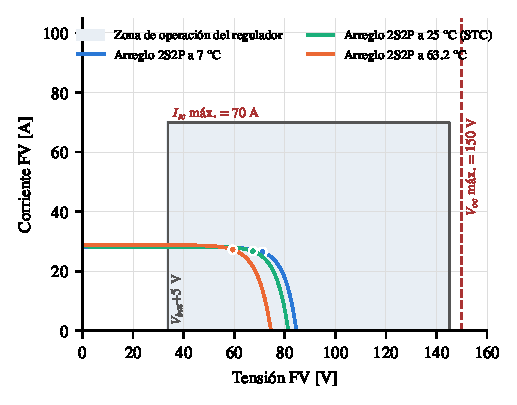
\includegraphics[width=\anchofig]{soa_regulador.pdf}
\caption{Zona de operación del regulador y curvas I-V del arreglo 2S2P a distintas temperaturas de celda. Los puntos marcan la máxima potencia.}
\label{fig:soa}
\end{figure}

\subsection{Inversor-cargador}

El inversor de un sistema aislado se dimensiona con la potencia de las cargas de alterna que funcionan a la vez, debe soportar los picos de arranque de los motores, que pueden ser de 3 a 4 veces la potencia nominal, y debe tener corte por baja tensión del banco. La tensión de entrada es la del banco y la de salida, la de las cargas. Con las cargas críticas, la potencia simultánea es de \SI{783}{W} y el pico con el arranque de los dos compresores, de \SI{1763}{W} (Sección~\ref{sec:lugar}).

Se seleccionó el inversor-cargador Victron MultiPlus-II 24/3000/70-50 de \SI{120}{V}, cuyas características están en la Tabla~\ref{tab:inversor}. Las cargas usan el 33\,\% de su potencia continua a \SI{25}{\celsius} y el 32\,\% de su potencia pico. Es el modelo de menor potencia de la serie MultiPlus-II para \SI{24}{V} y \SI{120}{V} \cite{victron_mp}. Incluye un conmutador de transferencia de \SI{50}{A}: si falla la red, pasa las cargas al inversor en menos de \SI{20}{ms}, de modo que los equipos electrónicos siguen funcionando sin interrupción. También incluye un cargador de \SI{70}{A}, que puede recargar el banco desde la red cuando la energía solar no alcanza, y protección por baja tensión del banco \cite{victron_mp}. Su salida es de onda senoidal, apta para los compresores y para los equipos electrónicos.

\begin{table}[!htb]
\caption{Inversor-cargador Victron MultiPlus-II 24/3000/70-50 120V \cite{victron_mp} frente a las cargas}
\label{tab:inversor}
\centering
\footnotesize
\setlength{\tabcolsep}{3pt}
\begin{tabular}{l l l}
\toprule
Parámetro & Cargas críticas & Inversor-cargador \\
\midrule
Potencia continua & \SI{783}{W} & \SI{2400}{W} a \SI{25}{\celsius}; \SI{2200}{W} a \SI{40}{\celsius} \\
Potencia pico & \SI{1763}{W} & \SI{5500}{W} \\
Tensión de entrada DC & \SI{24}{V} & 19 a \SI{33}{V} \\
Salida AC & \SI{120}{V}, \SI{60}{Hz} & \SI{120}{V} $\pm$ 2\,\%, \SI{60}{Hz} \\
Corriente de batería & \SI{34.3}{A} (\SI{77.3}{A} en el arranque) & \\
Conmutador de transferencia & & \SI{50}{A}, menos de \SI{20}{ms} \\
Cargador desde la red & & \SI{70}{A}; absorción \SI{28.8}{V}, flotación \SI{27.6}{V} \\
Eficiencia máxima & & 94\,\% \\
Consumo sin carga & & \SI{13}{W} (\SI{3}{W} en modo de búsqueda) \\
Temperatura de operación & & $-40$ a \SI{60}{\celsius} \\
Masa & & \SI{19}{kg} \\
\bottomrule
\end{tabular}
\end{table}

El consumo sin carga del inversor, de \SI{13}{W}, equivale a \SI{312}{Wh} por día si funciona sin interrupción, más que los \SI{217}{Wh} por día que representa la pérdida de 5\,\% del inversor en el balance. La diferencia, de \SI{95}{Wh} por día, queda cubierta por el excedente de \SI{697}{Wh} por día de noviembre (Tabla~\ref{tab:energia}), y se reduce si se activa el modo de búsqueda del equipo, de \SI{3}{W}.

\subsection{Estimación energética}

La energía diaria disponible para las cargas se estimó para cada mes como $E = P_{\mathrm{campo}}\cdot\mathrm{HSP}\cdot K_{TCA}$, con los \SI{1.8}{kW} del arreglo, la irradiación de la cara este y el mismo factor de rendimiento del balance. La Tabla~\ref{tab:energia} y la Fig.~\ref{fig:energia} comparan esa energía con la demanda de las cargas críticas.

\begin{table}[!htb]
\caption{Energía mensual disponible y demanda de las cargas críticas}
\label{tab:energia}
\centering
\footnotesize
\setlength{\tabcolsep}{4pt}
\begin{tabular}{l c r r r r}
\toprule
Mes & HSP & Generada [kWh] & Disponible [kWh] & Demanda [kWh] & Cobertura \\
\midrule
Ene & 5.03 & 280.7 & 210.3 & 134.4 & 156\,\% \\
Feb & 5.73 & 288.8 & 216.3 & 121.4 & 178\,\% \\
Mar & 5.94 & 331.5 & 248.3 & 134.4 & 185\,\% \\
Abr & 5.54 & 299.2 & 224.1 & 130.0 & 172\,\% \\
May & 4.55 & 253.9 & 190.2 & 134.4 & 142\,\% \\
Jun & 4.36 & 235.4 & 176.4 & 130.0 & 136\,\% \\
Jul & 4.35 & 242.7 & 181.8 & 134.4 & 135\,\% \\
Ago & 4.51 & 251.7 & 188.5 & 134.4 & 140\,\% \\
Set & 4.49 & 242.5 & 181.6 & 130.0 & 140\,\% \\
Oct & 3.94 & 219.9 & 164.7 & 134.4 & 123\,\% \\
Nov & 3.73 & 201.4 & 150.9 & 130.0 & 116\,\% \\
Dic & 4.46 & 248.9 & 186.4 & 134.4 & 139\,\% \\
\midrule
Año & & 3096 & 2320 & 1582 & 147\,\% \\
\bottomrule
\end{tabular}
\\[2pt]
{\footnotesize Generada: $P_{\mathrm{campo}}\cdot\mathrm{HSP}\cdot\text{días}$. Disponible: generada por $K_{TCA}=0.749$.}
\end{table}

\begin{figure}[!htb]
\centering
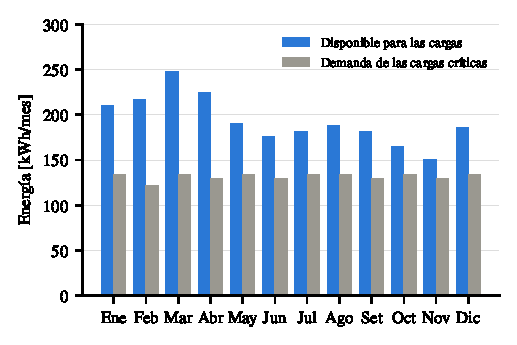
\includegraphics[width=\anchofig]{energia_mensual.pdf}
\caption{Energía mensual disponible para las cargas y demanda de las cargas críticas.}
\label{fig:energia}
\end{figure}

Todos los meses la energía disponible supera la demanda: en noviembre, el mes de diseño, la cobertura es de 116\,\%, y en marzo llega a 185\,\%. En el año hay \SI{2320}{kWh} disponibles para \SI{1582}{kWh} de demanda. El excedente no se aprovecha, porque el sistema no entrega energía a la red, pero permite recargar el banco después de días nublados: en noviembre el excedente medio es de \SI{0.70}{kWh} por día, de modo que recargar los \SI{13.44}{kWh} de los dos días de autonomía tomaría unos 19 días de radiación media, o menos si se usa el cargador desde la red. Como comparación, PVGIS estima para \SI{1.8}{kWp} en la cara este, con 14\,\% de pérdidas del sistema y las pérdidas por temperatura y ángulo de incidencia, \SI{2401}{kWh} al año y \SI{156}{kWh} en noviembre \cite{pvgis}, valores cercanos a la energía disponible estimada.

\section{Elementos de la instalación}\label{sec:instalacion}

\subsection{Estructura de montaje}

Los cuatro módulos se colocan en una fila, en vertical, sobre la cara este del techo y paralelos a la lámina, con la misma inclinación de \SI{12}{\degree}. Se usan dos rieles de aluminio Unirac SM, uno por cada mitad del módulo, sujetos a las clavadoras del techo con soportes tipo L atornillados a través de la lámina ondulada, con arandela y sello en cada perforación. Los módulos se fijan a los rieles con grapas intermedias, que además unen eléctricamente el marco al riel para la puesta a tierra, y con grapas de extremo. La Tabla~\ref{tab:montaje} presenta la lista de materiales.

\begin{table}[!htb]
\caption{Materiales de la estructura de montaje (una fila de 4 módulos)}
\label{tab:montaje}
\centering
\footnotesize
\setlength{\tabcolsep}{3pt}
\begin{tabular}{l l r}
\toprule
Elemento & Referencia & Cant. \\
\midrule
Riel de aluminio de \SI{6.1}{m}, cortado a \SI{4.7}{m} & Unirac \textit{SM Rail} 240" & 2 \\
Grapa intermedia con unión a tierra & Unirac \textit{SM BND Midclamp} & 6 \\
Grapa de extremo & Unirac \textit{SM Endclamp} & 4 \\
Soporte tipo L, con tornillo y sello a la clavadora & Unirac \textit{L-Foot} & 10 \\
Terminal de tierra para riel & \textit{Lay-in lug} & 2 \\
\bottomrule
\end{tabular}
\end{table}

La cantidad de soportes se estimó con uno cada \SI{1.2}{m} de riel, cinco por riel. La separación final depende de la distancia entre las clavadoras del techo, que debe medirse en el sitio. Los módulos y la estructura agregan unos \SI{90}{kg} sobre \SI{8}{m^2} de techo, unos \SI{11}{kg/m^2}; falta verificar con el grupo el estado de las clavadoras y de la lámina antes de la instalación.

\subsection{Cableado}

Las longitudes de los tramos son supuestas, porque aún no se ha definido la ruta: \SI{10}{m} desde los módulos hasta los equipos, \SI{1.5}{m} entre la caja combinadora, el regulador y la barra DC, \SI{1}{m} entre cada batería y la barra, \SI{2}{m} entre la barra y el inversor, y \SI{5}{m} entre el inversor y los tableros. La corriente de diseño se calculó como $i_w=1.25\cdot1.25\cdot I_{sc}$ en los circuitos fotovoltaicos y como $i_w=1.25\cdot I_{\max}$ en los demás. Para el inversor, $I_{\max}$ es la corriente DC a su potencia continua, $2400/(0.94\cdot22.4)=\SI{114}{A}$, con \SI{22.4}{V} como tensión del banco casi descargado (\SI{2.8}{V} por celda, supuesto) \cite{nec2014}. La capacidad de los conductores se tomó de la Tabla 310.15(B)(16) del NEC 2014, la edición oficializada en Costa Rica \cite{codigo_electrico, nec2014}, y la caída de tensión se calculó con
\begin{equation}
\Delta V = 2\,L\,I\,R,
\end{equation}
donde $L$ es la longitud del tramo, $I$ la corriente y $R$ la resistencia del conductor por unidad de longitud (NEC, Cap.~9, Tabla 8). La Tabla~\ref{tab:cables} presenta el resultado.

\begin{table}[!htb]
\caption{Conductores por tramo}
\label{tab:cables}
\centering
\footnotesize
\setlength{\tabcolsep}{2.5pt}
\begin{tabular}{c l c c c c c}
\toprule
Tramo & Recorrido & $L$ [m] & $i_w$ [A] & Conductor & Capacidad [A] & $\Delta V$ [\%] \\
\midrule
T1 & Cadena -- caja combinadora & 10 & 22.5 & 10 AWG PV Wire & 26.2 & 1.82 \\
T2 & Caja combinadora -- regulador & 1.5 & 45.0 & 8 AWG THHN & 50 & 0.35 \\
T3 & Regulador -- barra DC & 1.5 & 106.2 & 2 AWG & 115 & 0.67 \\
T4 & Batería -- barra DC (cada una) & 1 & 96.9 & 2 AWG & 115 & 0.41 \\
T5 & Barra DC -- inversor & 2 & 142.5 & 2/0 AWG & 175 & 0.60 \\
T6 & Tablero principal -- inversor & 5 & 31.2 & 8 AWG THHN & 50 & 0.52 \\
T7 & Inversor -- subtablero crítico & 5 & 31.2 & 8 AWG THHN & 50 & 0.52 \\
\bottomrule
\end{tabular}
\\[2pt]
{\footnotesize $\Delta V$: T1 y T2 con $I_{mp}$ y $V_{mp}$ a \SI{63.2}{\celsius}; T3 con \SI{85}{A}; T4 con el doble de la parte de una batería; T5 con \SI{114}{A}; T6 y T7 con \SI{25}{A} a \SI{120}{V}.}
\end{table}

En el tramo T1 la corriente de diseño es $1.25\cdot1.25\cdot\SI{14.39}{A}=\SI{22.5}{A}$, con la $I_{sc}$ a \SI{63.2}{\celsius}. Se usa \textit{PV Wire} de 10 AWG, que admite \SI{40}{A} a \SI{90}{\celsius}; con las dos cadenas en una sola canalización (4 conductores, factor 0.80) y una temperatura sobre el techo de hasta \SI{50}{\celsius} (factor 0.82), su capacidad es de \SI{26.2}{A}. En T2 las dos cadenas ya están en paralelo y $i_w=\SI{45.0}{A}$. En T3 se usa la corriente máxima del regulador, \SI{85}{A}, y el calibre 2 AWG es el mayor que admiten sus terminales \cite{victron_mppt}. En T4, la corriente máxima del banco, \SI{155}{A}, es la carga simultánea del regulador y del cargador del inversor; cada batería lleva un cuarto, y por si el reparto no es parejo se dimensionó con el doble, \SI{77.5}{A}. Los cuatro cables T4 deben tener la misma longitud para que las baterías se repartan la corriente. En T5, $i_w=1.25\cdot\SI{114}{A}=\SI{142.5}{A}$, y el 2/0 AWG admite \SI{175}{A}. En la parte de corriente alterna, la corriente máxima del inversor es $\SI{3000}{VA}/\SI{120}{V}=\SI{25}{A}$.

La caída de tensión del lado fotovoltaico, sumando T1, T2 y T3, es de 2.84\,\%, y la del lado de alterna, de 0.52\,\% por tramo. Las dos quedan por debajo del 3\,\% por circuito que recomienda el NEC \cite{nec2014}. El tramo T1 es el de mayor caída; si la distancia real supera los \SI{10}{m}, conviene usar 8 AWG.

\subsection{Protecciones}

La Tabla~\ref{tab:protecciones} presenta las protecciones. Con solo dos cadenas no se requieren fusibles de cadena: si una cadena falla, la corriente inversa máxima que recibe es la de la otra, $1.25\cdot\SI{14.12}{A}=\SI{17.7}{A}$, menor que los \SI{25}{A} del fusible máximo en serie del módulo \cite{aiko_ds, nec2014}. En la entrada fotovoltaica del regulador se instala un protector de falla a tierra con interruptor, que sirve además como medio de desconexión del arreglo, y en la caja combinadora un descargador de sobretensiones de \SI{115}{V}, mayor que los \SI{84.6}{V} del arreglo en frío.

En el lado de las baterías, cada batería tiene su interruptor de \SI{100}{A}, que protege su conductor de 2 AWG (\SI{115}{A}) y permite desconectarla sin apagar el sistema. El interruptor de la salida del regulador es de \SI{125}{A}, el valor normalizado siguiente a la capacidad de \SI{115}{A} del conductor, como permite el NEC \cite{nec2014}, y el de la entrada del inversor es de \SI{175}{A}, igual a la capacidad del 2/0 AWG. La corriente del banco durante el arranque de los compresores, \SI{77.3}{A}, es menor que la de cualquiera de estos interruptores. En el lado de alterna, la entrada del inversor se alimenta desde un interruptor de \SI{40}{A} en el tablero principal, y el subtablero de cargas críticas tiene un interruptor principal de \SI{40}{A}; los circuitos existentes de refrigeración, iluminación y tomas se trasladan a ese subtablero con sus propios interruptores.

\begin{table}[!htb]
\caption{Lista de protecciones}
\label{tab:protecciones}
\centering
\footnotesize
\setlength{\tabcolsep}{3pt}
\begin{tabular}{l l c}
\toprule
Ubicación & Protección & Cant. \\
\midrule
Caja combinadora & Descargador DC MidNite MNSPD-115 & 1 \\
Entrada FV del regulador & Protector de falla a tierra MidNite MNDC-GFP80 (\SI{80}{A}, \SI{150}{V}) & 1 \\
Salida del regulador & Interruptor DC MidNite MNEDC125 (\SI{125}{A}) & 1 \\
Cada batería & Interruptor DC MidNite MNEDC100 (\SI{100}{A}, \SI{150}{V}) & 4 \\
Entrada DC del inversor & Interruptor DC MidNite MNEDC175 (\SI{175}{A}, \SI{125}{V}) & 1 \\
Inversor & Corte por baja tensión, sobrecarga y cortocircuito (integrados) & -- \\
Tablero principal & Interruptor 1P \SI{40}{A} Square D QO140 & 1 \\
Subtablero crítico & Interruptor principal 1P \SI{40}{A} Square D QO140 & 1 \\
Puesta a tierra & Marcos, rieles, gabinetes y polo negativo del banco, Cu 8 AWG & -- \\
\bottomrule
\end{tabular}
\end{table}

\subsection{Diagrama unifilar}

La Fig.~\ref{fig:unifilar} presenta el diagrama unifilar del sistema con la simbología de la norma IEC 60617.

\begin{sidewaysfigure}
\centering
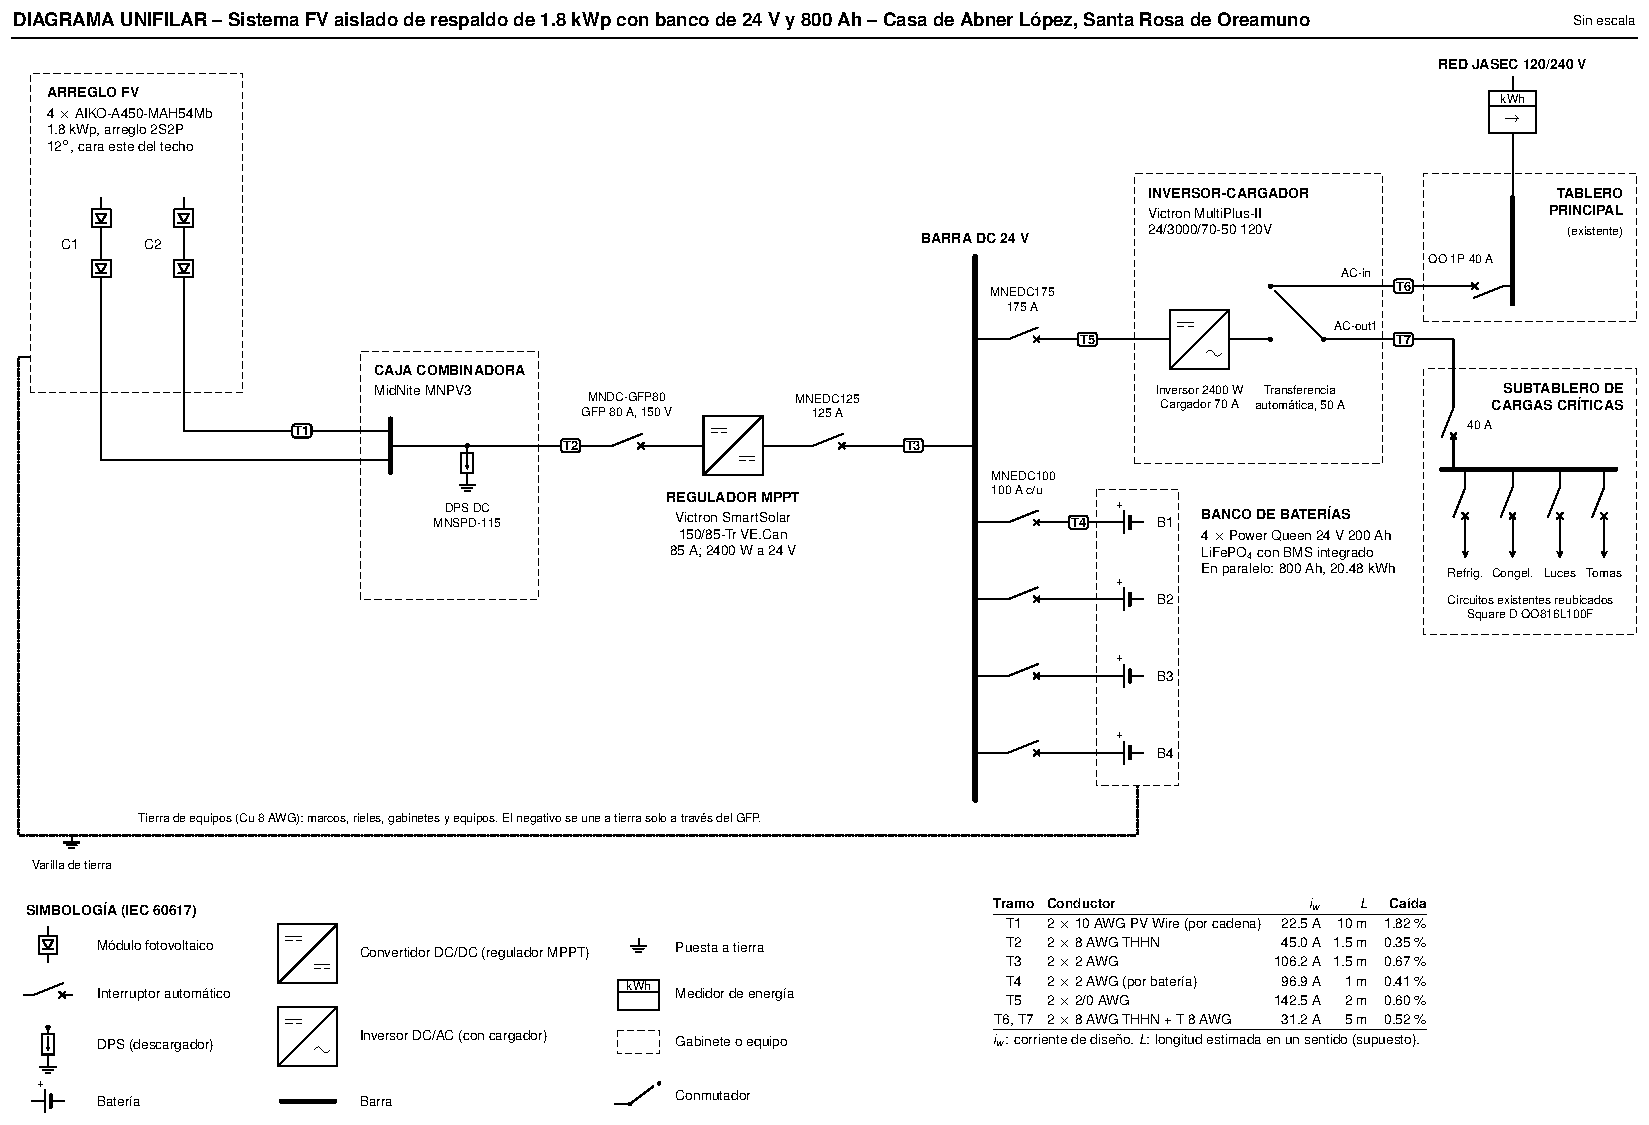
\includegraphics[width=\textheight]{unifilar_tikz.pdf}
\caption{Diagrama unifilar del sistema aislado de respaldo.}
\label{fig:unifilar}
\end{sidewaysfigure}

\section{Evaluación económica}\label{sec:economia}

\subsection{Costo del sistema}

El costo incluye los equipos, la estructura, los conductores, las protecciones, el diseño y la instalación (Tabla~\ref{tab:costos}). Las baterías se valoraron con el precio de Costa Rica \cite{kuat}; para los demás equipos no se encontraron precios publicados en el país, por lo que se usaron precios de lista de tiendas de Estados Unidos y Europa de octubre y noviembre de 2026 \cite{precio_modulo, precio_mppt, precio_mp, pes, elliott, standard, zoro}. Los dólares y euros se convirtieron con el tipo de cambio de referencia de venta del BCCR del 19 de noviembre de 2026, ¢447.54 por dólar, y 1.0997 dólares por euro \cite{bccr}. Las canalizaciones, los conductores de puesta a tierra y los accesorios se estimaron como un 15\,\% de los conductores y protecciones. Para el diseño se usaron los honorarios mínimos del arancel del CFIA, 4.5\,\% del valor de la obra \cite{cfia_arancel}, y para el registro del proyecto, 0.25\,\% \cite{cfia_registro}. Para la instalación no se encontraron valores públicos en Costa Rica, así que se supusieron ¢300\,000 de mano de obra y un 20\,\% de ganancia del instalador sobre el costo total.

\begin{table}[!htb]
\caption{Costo estimado del sistema}
\label{tab:costos}
\centering
\footnotesize
\setlength{\tabcolsep}{4pt}
\begin{tabular}{l r}
\toprule
Rubro & Monto [¢] \\
\midrule
Baterías Power Queen 24 V 200 Ah (4 $\times$ ¢850\,000) & 3\,400\,000 \\
Inversor-cargador MultiPlus-II (997.05 USD) & 446\,220 \\
Módulos AIKO 450 W (4 $\times$ 128.96 EUR) & 253\,876 \\
Regulador SmartSolar 150/85 (476.00 USD) & 213\,029 \\
Estructura de montaje (Tabla~\ref{tab:montaje}) & 134\,978 \\
Conductores & 279\,318 \\
Protecciones y tableros (Tabla~\ref{tab:protecciones}) & 505\,998 \\
Otros materiales eléctricos (15\,\%) & 117\,797 \\
\midrule
Subtotal de equipos y materiales & 5\,351\,216 \\
\midrule
Diseño, honorarios CFIA (4.5\,\%) & 254\,305 \\
Registro ante el CFIA (0.25\,\%) & 14\,128 \\
Instalación (supuesto) & 300\,000 \\
\midrule
Costo total & 5\,919\,648 \\
Ganancia del instalador (20\,\%) & 1\,183\,930 \\
\midrule
\textbf{Precio del sistema} & \textbf{7\,103\,578} \\
\bottomrule
\end{tabular}
\\[2pt]
{\footnotesize Equivale a 15\,872 USD. No incluye flete, nacionalización ni IVA de los equipos importados. Las partidas están redondeadas al colón.}
\end{table}

Las baterías son el 48\,\% del precio. El costo real puede ser mayor, porque no se incluyeron el flete ni los impuestos de importación de los equipos, y debe confirmarse con cotizaciones de distribuidores locales.

\subsection{Ahorro en la factura}

Con el sistema, las cargas críticas dejan de tomar energía de la red, porque la energía disponible cubre su demanda todos los meses (Tabla~\ref{tab:energia}). La factura con el sistema se calculó con la misma tarifa (Tabla~\ref{tab:tarifa}), restando al consumo de cada mes la energía de las cargas críticas (Tabla~\ref{tab:facturas}). La factura anual baja de ¢236\,730 a ¢108\,565, un ahorro de ¢128\,165 (54\,\%). El ahorro es mayor que la proporción de energía, de 49\,\%, porque al bajar el consumo de unos \SI{270}{kWh} a unos \SI{140}{kWh} por mes desaparecen el bloque de ¢76.02/kWh y el IVA de los meses que superaban \SI{280}{kWh}. Este ahorro supone que el sistema funciona todos los días, no solo durante los cortes; si se usara solo como respaldo, el ahorro se limitaría a la energía consumida durante los cortes.

\subsection{Proyección financiera}

El flujo de caja se proyectó a 25 años con una tasa de descuento de 7\,\% y tarifas constantes. La degradación de los módulos, de 1\,\% el primer año y 0.35\,\% por año después \cite{aiko_ds}, no reduce el ahorro: en el año 25 la energía disponible baja 9.4\,\% y la cobertura de noviembre queda en 105\,\%, de modo que las cargas críticas se siguen cubriendo. Se supuso un mantenimiento de 1\,\% del precio por año (¢71\,036) y el reemplazo del inversor y el regulador en el año 13 (¢659\,249), porque sus fichas no declaran la vida útil. Las baterías se reemplazan en el año 15 (¢3\,400\,000): con una descarga diaria de 22\,\%, los 15\,000 ciclos que declara el fabricante al 60\,\% de DOD \cite{pq} no limitan su vida, pero el fabricante no declara la vida calendario.

\begin{figure}[!htb]
\centering
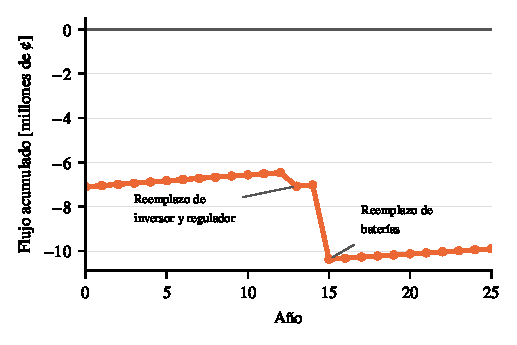
\includegraphics[width=\anchofig]{flujo_acumulado.pdf}
\caption{Flujo de caja acumulado del sistema.}
\label{fig:flujo}
\end{figure}

La Fig.~\ref{fig:flujo} muestra el flujo acumulado. El ahorro anual, ¢128\,165, supera el mantenimiento en ¢57\,129, de modo que el flujo acumulado sube unos ¢57\,000 por año, y los reemplazos lo bajan a ¢10.31 millones negativos en el año 15. Al final de los 25 años el flujo acumulado es de ¢9.73 millones negativos y el valor actual neto, de ¢7.94 millones negativos: la inversión no se recupera. Sin mantenimiento ni reemplazos, el tiempo de recuperación simple sería de $7\,103\,578/128\,165=55$ años.

El costo de la energía que entrega el sistema a las cargas críticas, calculado como el valor presente de los costos entre el valor presente de la energía, es de ¢512/kWh, frente al costo de la energía de la red en el bloque de más de \SI{200}{kWh}, de ¢76.02/kWh más alumbrado, bomberos e IVA. El resultado indica que el sistema no se justifica por el ahorro en la factura: su valor está en mantener funcionando la refrigeración, la iluminación y las comunicaciones durante dos días sin servicio eléctrico.

\section{Conclusiones}

Las cargas críticas de la vivienda, refrigerador, congelador, iluminación, cargadores y módem, consumen \SI{4.33}{kWh} por día y piden \SI{783}{W} si todas funcionan a la vez. Con el método del curso, dos días de autonomía, \SI{24}{V} y 70\,\% de descarga, el banco requiere \SI{758}{Ah}, que se cubren con cuatro baterías Power Queen LiFePO\textsubscript{4} de \SI{200}{Ah} en paralelo, el máximo que admite el fabricante.

La cara este del techo, de \SI{12}{\degree}, recibe \SI{1720}{kWh/m^2} al año, 6.5\,\% más que la cara oeste; el plano óptimo recibiría 1.7\,\% más. Con los \SI{3.73}{HSP} de noviembre, el peor mes, se requieren cuatro módulos AIKO de \SI{450}{W}, que se conectan en dos cadenas de dos para cumplir los límites de tensión del regulador entre 7 y \SI{63.2}{\celsius}.

El regulador Victron SmartSolar 150/85 cumple la corriente de \SI{75}{A} que pide el método del curso, y el inversor-cargador Victron MultiPlus-II de \SI{3000}{VA} trabaja al 33\,\% de su potencia continua y al 32\,\% de su pico; si falla la red, conmuta las cargas a su inversor en menos de \SI{20}{ms}.

La energía disponible para las cargas supera la demanda todos los meses: en noviembre la cobertura es de 116\,\%, y en el año hay \SI{2319}{kWh} disponibles para \SI{1582}{kWh} de demanda.

El sistema cuesta unos ¢7.10 millones, de los cuales el 48\,\% son las baterías. Reduce la factura en ¢128\,165 al año (54\,\%), pero con el mantenimiento y los reemplazos la inversión no se recupera en 25 años (VAN de ¢8.00 millones negativos). Su justificación es la continuidad del servicio de las cargas críticas, no el ahorro.

Antes de construir deben confirmarse los precios con distribuidores locales, las distancias de los tramos de cableado, la separación y el estado de las clavadoras del techo y la reducción de potencia del regulador por la altitud del sitio.


\section*{Herramientas de apoyo}

Durante el proyecto se utilizó inteligencia artificial para revisar partes de la redacción y ayudar a preparar algunas gráficas, diagramas y scripts de cálculo. Antes de incluir los resultados en el informe, fueron revisados con los datos del sitio y las especificaciones de los equipos. La configuración propuesta y las conclusiones fueron decisiones del grupo.

\begin{thebibliography}{99}
\bibitem{aresep_tre} Autoridad Reguladora de los Servicios Públicos, ``Datos abiertos: tarifas de distribución de electricidad, JASEC, tarifa residencial T-RE, 2026,'' resolución RE-0072-IE-2025, \textit{La Gaceta} N.\textsuperscript{o} 236, Alcance 161, 16 dic. 2025. [En línea]. Disponible: \url{https://datos.aresep.go.cr/ws.datosabiertos/Services/IE/TarifasElectricidad.svc/ObtenerTarifasElectricidadDistribucion/0}. Consultado: 19 nov. 2026.
\bibitem{aresep_ap} Autoridad Reguladora de los Servicios Públicos, ``Datos abiertos: tarifas de alumbrado público, JASEC, 2026,'' resolución RE-0072-IE-2025. [En línea]. Disponible: \url{https://datos.aresep.go.cr/ws.datosabiertos/Services/IE/TarifasElectricidad.svc/ObtenerTarifasElectricidadAlumbradoPublico/0}. Consultado: 19 nov. 2026.
\bibitem{ley8992} Costa Rica, Ley N.\textsuperscript{o} 8992, ``Fortalecimiento del Cuerpo de Bomberos,'' 2011.
\bibitem{ley9635} Costa Rica, Ley N.\textsuperscript{o} 9635, ``Fortalecimiento de las finanzas públicas,'' 2018.
\bibitem{pvgis} European Commission, Joint Research Centre, ``Photovoltaic Geographical Information System (PVGIS) v5.3, base PVGIS-ERA5 2005--2023,'' [En línea]. Disponible: \url{https://re.jrc.ec.europa.eu/pvg_tools/en/}. Consultado: 9 oct. 2026.
\bibitem{aiko_ds} AIKO, ``Neostar 2S AIKO-A-MAH54Mb, 440--470 W: hoja de datos,'' versión V6.3. [En línea]. Disponible: \url{https://www.solartraders.com/uploads/production/data_sheet/file/37607/data_sheet_aiko_a_mah54mb_glas_folie_neostar_2s_de_01-12-2024.pdf}. Consultado: 9 oct. 2026.
\bibitem{trojan_t105} Trojan Battery Company, ``Data sheet: Motive T-105,'' T-105.DS\_020819, 2019. [En línea]. Disponible: \url{https://assets.ctfassets.net/nh2mdhlonj7m/3RwDBLAA3SCrYnhfDrQnKl/01b3929a9ced420254efa6ced4fb9ab4/T105_Trojan_Data_Sheets.pdf}. Consultado: 5 nov. 2026.
\bibitem{trojan_sig} Trojan Battery Company, ``Signature Line: deep-cycle flooded batteries,'' folleto, documento alojado por un distribuidor. [En línea]. Disponible: \url{https://www.battery.cz/user/related_files/signature_line.pdf}. Consultado: 5 nov. 2026.
\bibitem{trojan_saes} Trojan Battery Company, ``Data sheet: Solar SAES 12 205,'' 2023. [En línea]. Disponible: \url{https://assets.ctfassets.net/nh2mdhlonj7m/6DxgAAohXEqPFkjGlXk8UF/a20a36c1776d4bdade8e4fb2bf5e2608/202307-SAES-12-205-Datasheet-WEB.pdf}. Consultado: 5 nov. 2026.
\bibitem{ultracell} Ultracell, ``UCG200-12: 12V 200Ah gel battery, technical data,'' ficha técnica alojada por un distribuidor. [En línea]. Disponible: \url{https://www.solaris-store.com/telechargement/fiche/Fiche-technique-Batterie-ultracell-UCG200.pdf}. Consultado: 5 nov. 2026.
\bibitem{pq} Power Queen, ``Power Queen 24V 200Ah deep cycle LiFePO4 lithium battery,'' especificaciones y precio del producto. [En línea]. Disponible: \url{https://ipowerqueen.com/products/power-queen-24v-200ah-lifepo4-battery}. Consultado: 12 nov. 2026.
\bibitem{victron_ds} Victron Energy, ``12,8 \& 25,6 Volt lithium-iron-phosphate batteries Smart,'' hoja de datos. [En línea]. Disponible: \url{https://www.victronenergy.com/upload/documents/Datasheet-12,8-&-25,6-Volt-lithium-iron-phosphate-batteries-Smart-EN.pdf}. Consultado: 5 nov. 2026.
\bibitem{kuat} KUAT Costa Rica, ``Power Queen 24V 200Ah.'' [En línea]. Disponible: \url{https://kuatcr.com/product/power-queen-24v-200ah/}. Consultado: 12 nov. 2026.
\bibitem{pq_manual} Power Queen, ``Product manual: 25.6V 200Ah lithium iron phosphate (LiFePO4) battery.'' [En línea]. Disponible: \url{https://ipowerqueen.com/cdn/shop/files/24V_200Ah_Classic.pdf}. Consultado: 12 nov. 2026.
\bibitem{victron_mppt} Victron Energy, ``SmartSolar MPPT 150/70 up to 250/100 VE.Can: technical specifications,'' manual del producto. [En línea]. Disponible: \url{https://www.victronenergy.com/media/pg/Manual_SmartSolar_MPPT_150-70_up_to_250-100_VE.Can/en/technical-specifications.html}. Consultado: 20 nov. 2026.
\bibitem{victron_mp} Victron Energy, ``MultiPlus-II inverter/charger 120 V,'' hoja de datos. [En línea]. Disponible: \url{https://www.victronenergy.com/upload/documents/Datasheet-MultiPlus-II-120V-EN.pdf}. Consultado: 20 nov. 2026.
\bibitem{nec2014} National Fire Protection Association, \textit{NFPA 70: National Electrical Code}, ed. 2014. Quincy, MA, EE.\,UU.: NFPA, 2014.
\bibitem{codigo_electrico} Costa Rica, Decreto Ejecutivo N.\textsuperscript{o} 36979-MEIC, ``RTCR 458:2011 Reglamento de oficialización del Código Eléctrico de Costa Rica para la seguridad de la vida y de la propiedad,'' y sus reformas (Decreto 43418-MEIC).
\bibitem{precio_modulo} Cambio Energético, ``Panel solar AIKO Neostar 2S 450 W,'' [En línea]. Disponible: \url{https://www.cambioenergetico.com/producto/aiko-neostar-2s-450w/}. Consultado: nov. 2026.
\bibitem{precio_mppt} DRSA, ``Victron SmartSolar MPPT 150/85-Tr VE.Can SCC115085411,'' [En línea]. Disponible: \url{https://www.drsa.com/products/victron-smart-solar-mppt-150-85-tr-ve-can-scc115085411}. Consultado: nov. 2026.
\bibitem{precio_mp} DRSA, ``Victron MultiPlus-II 24/3000/70-50 120V UL PMP242305102,'' [En línea]. Disponible: \url{https://www.drsa.com/products/victron-multiplus-ii-24-3000-70-50-120v-ul-approved-pmp242305102}. Consultado: nov. 2026.
\bibitem{precios_bos} Precios consultados en noviembre de 2026 en PES Supply (\url{https://www.portlandiaelectric.supply}): MidNite MNEDC100, MNEDC125RT, MNEDC175, MNDC-GFP80, MNSPD-115, MNPV3, MNEDCQUAD y MNBIGBUSBAR; y en octubre de 2026: Unirac SM Rail, Midclamp, Endclamp, L-Foot y PV Wire 10 AWG. Elliott Electric Supply (\url{https://www.elliottelectric.com}): cable de cobre 1/0 y 2/0 AWG y THHN. Standard Electric Supply (\url{https://www.standardelectricsupply.com}): Square D QO140. Zoro (\url{https://www.zoro.com}): Square D QO816L100F.
\bibitem{bccr} Banco Central de Costa Rica, ``Tipo de cambio de referencia de venta (indicador 318) y euro (indicador 333),'' 19 nov. 2026. [En línea]. Disponible: \url{https://www.bccr.fi.cr/}. Consultado: 20 nov. 2026.
\bibitem{cfia_arancel} Costa Rica, Decreto Ejecutivo N.\textsuperscript{o} 18636-MOPT, ``Arancel de servicios profesionales de consultoría para edificaciones,'' \textit{La Gaceta} N.\textsuperscript{o} 225, 25 nov. 1988. [En línea]. Disponible: \url{https://cfia.or.cr/site/wp-content/uploads/2024/pdf/descargas/reglamentos/ejercicio/arancel-de-servicios-profesionales-de-consultoria-para-edificaciones.pdf}. Consultado: 11 oct. 2026.
\bibitem{cfia_registro} Colegio Federado de Ingenieros y de Arquitectos de Costa Rica, ``Registro de responsabilidad por consultorías varias,'' Centro de ayuda CFIA. [En línea]. Disponible: \url{https://centrodeayuda.cfia.or.cr/hc/es/articles/360025821333}. Consultado: 11 oct. 2026.
\end{thebibliography}

\end{document}
